\begin{figure}
  \centering \subfloat[][Well-fit: $z_1 = 20, z_2 = 45$.]{\noindent
    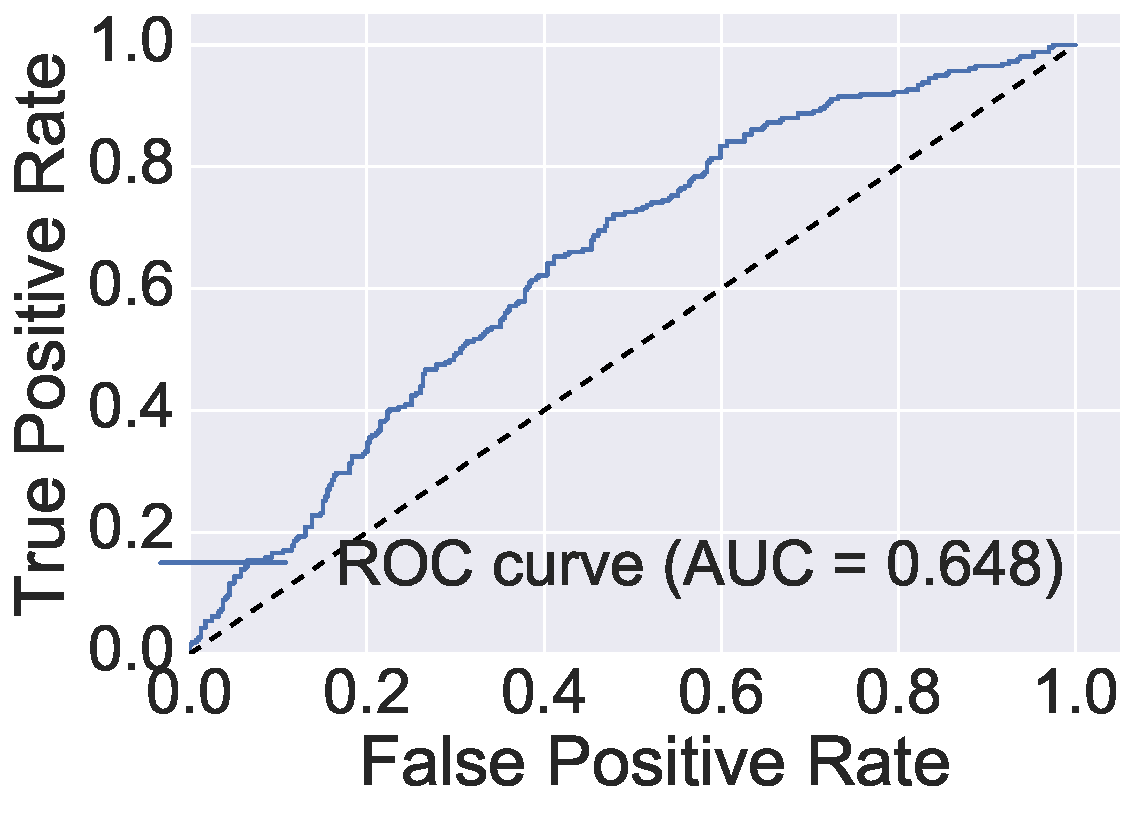
\includegraphics[width=.4\textwidth]{{/Users/ijoseph/Documents/Work/Graduate-Thesis/TeX/figures/ch4/cgp/mfaa_well_roc}.pdf}}%
  \qquad \\
  \subfloat[][Under-fit: $z_1 = 2, z_2 = 3$ .]{        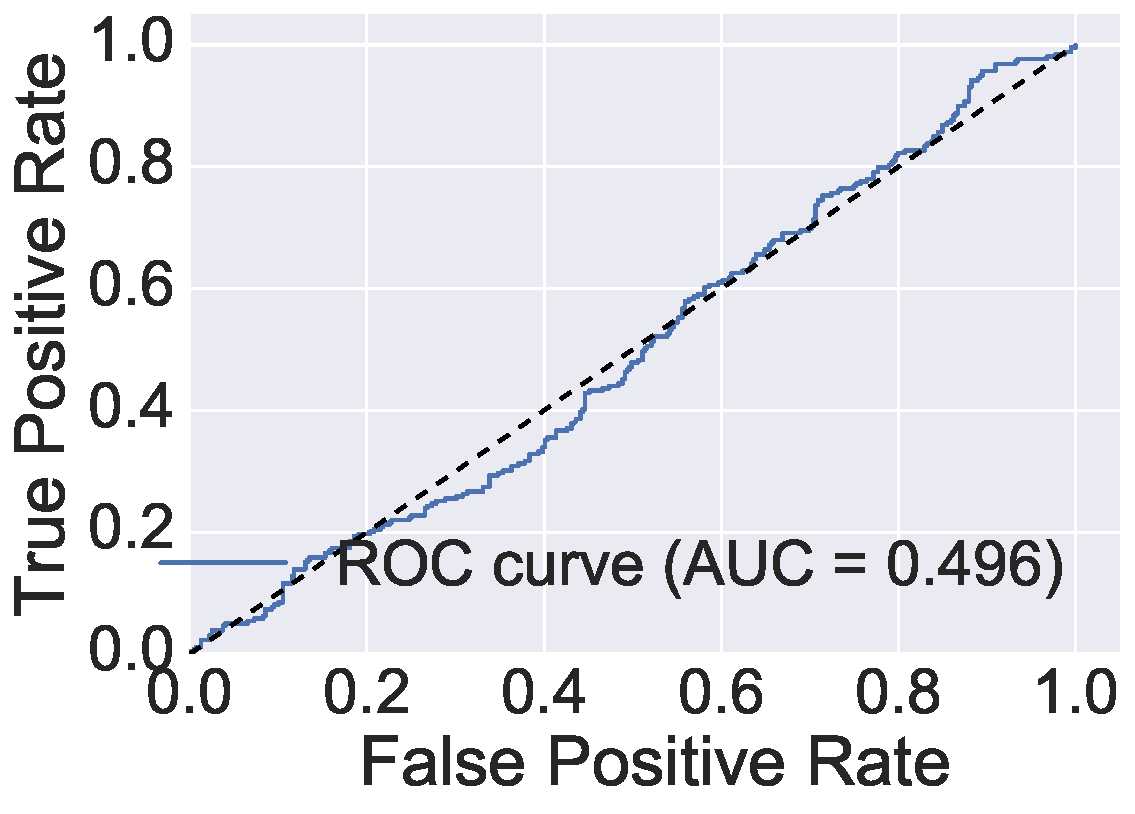
\includegraphics[width=.4\textwidth]{{/Users/ijoseph/Documents/Work/Graduate-Thesis/TeX/figures/ch4/cgp/mfaa_under_roc}.pdf}}%
  \qquad \\
\subfloat[][Closest to overfitting as possible: $z_1 = 62, z_2 =
65$. Note that the same AUC was the well-fit model was achieved at
this latent dimensionality. Higher latent dimensionality, which would
likely allow for AUC-degrading overfitting, was not possible as the
model currently is not implemented for latent dimensions higher than
the above.]{        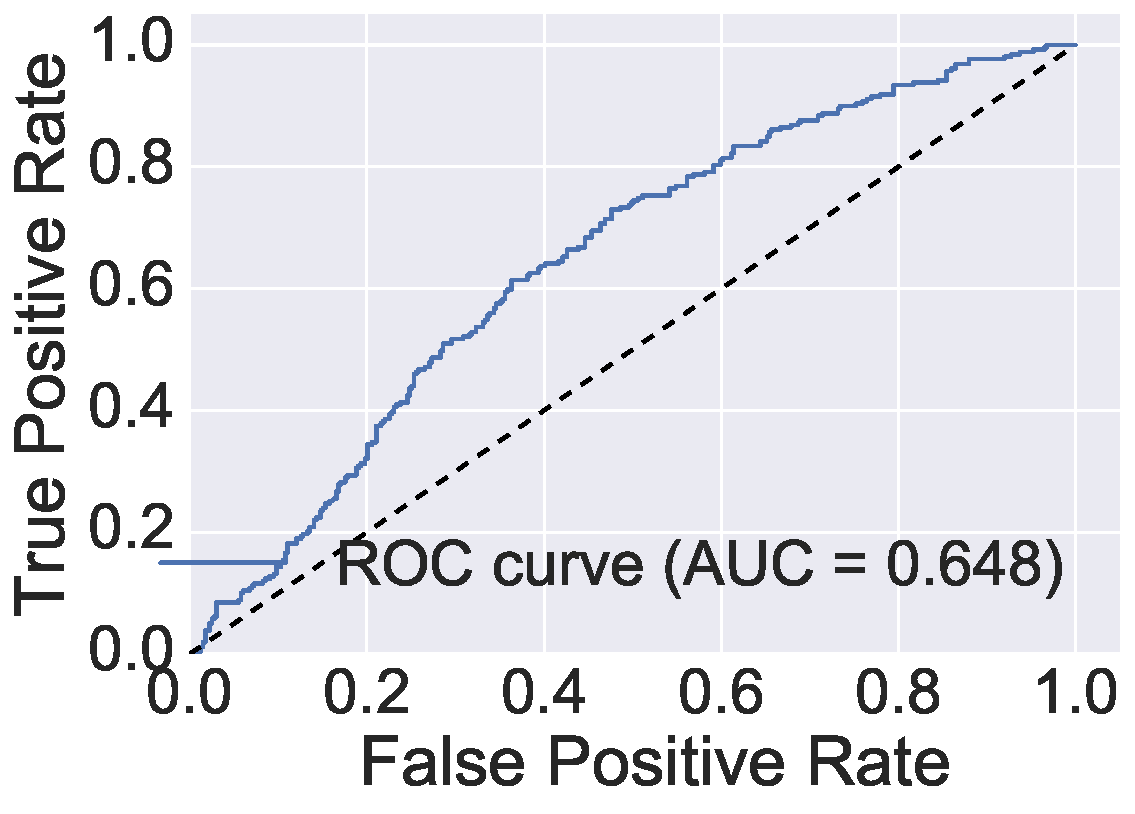
\includegraphics[width=.4\textwidth]{{/Users/ijoseph/Documents/Work/Graduate-Thesis/TeX/figures/ch4/cgp/mfaa_over_roc}.pdf}}%
  \caption{HFAM ROC curves for different levels of model
    complexity.} \label{fourcgpone}
\end{figure}
    

    \begin{figure} 
      \centering \subfloat[][Well-fit: $C = 1 \times 10^5$.]{\noindent
        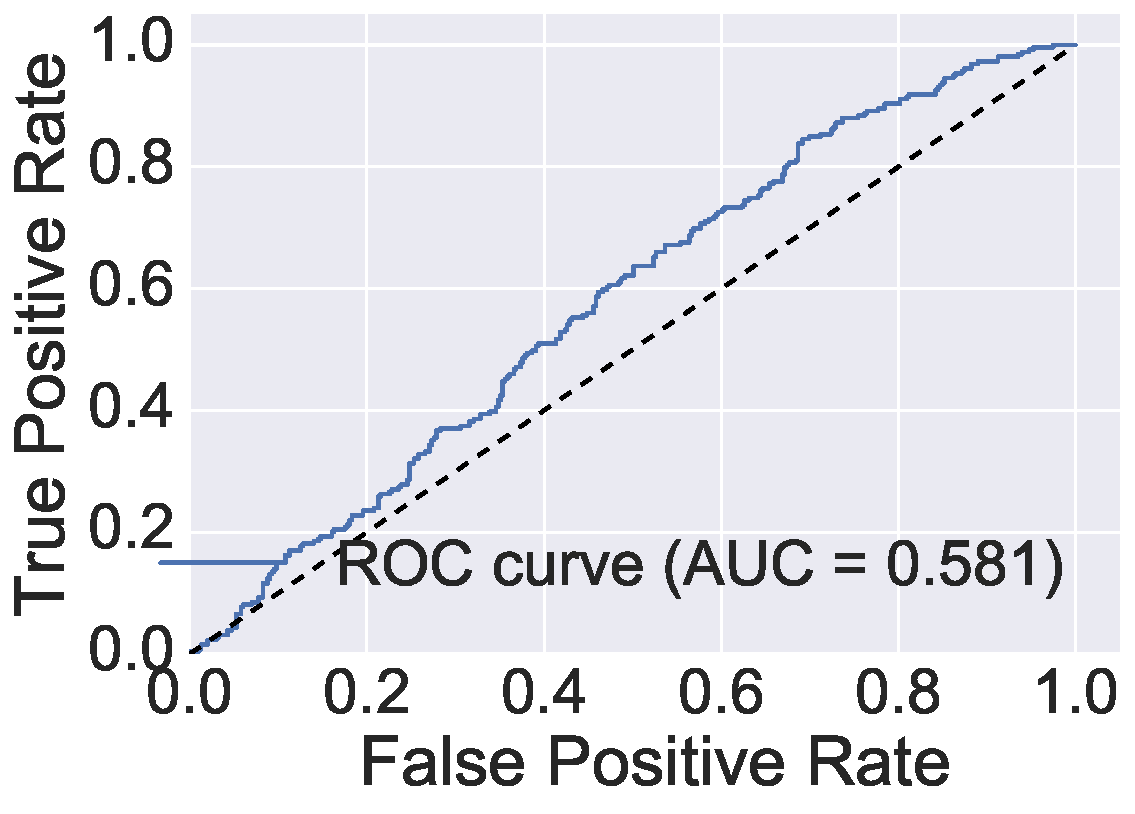
\includegraphics[width=.4\textwidth]{{/Users/ijoseph/Documents/Work/Graduate-Thesis/TeX/figures/ch4/cgp/log_reg_well_roc}.pdf}}%
      \qquad \\
      \subfloat[][Under-fit: $C = 1 \times 10^{-5}$
      .]{
        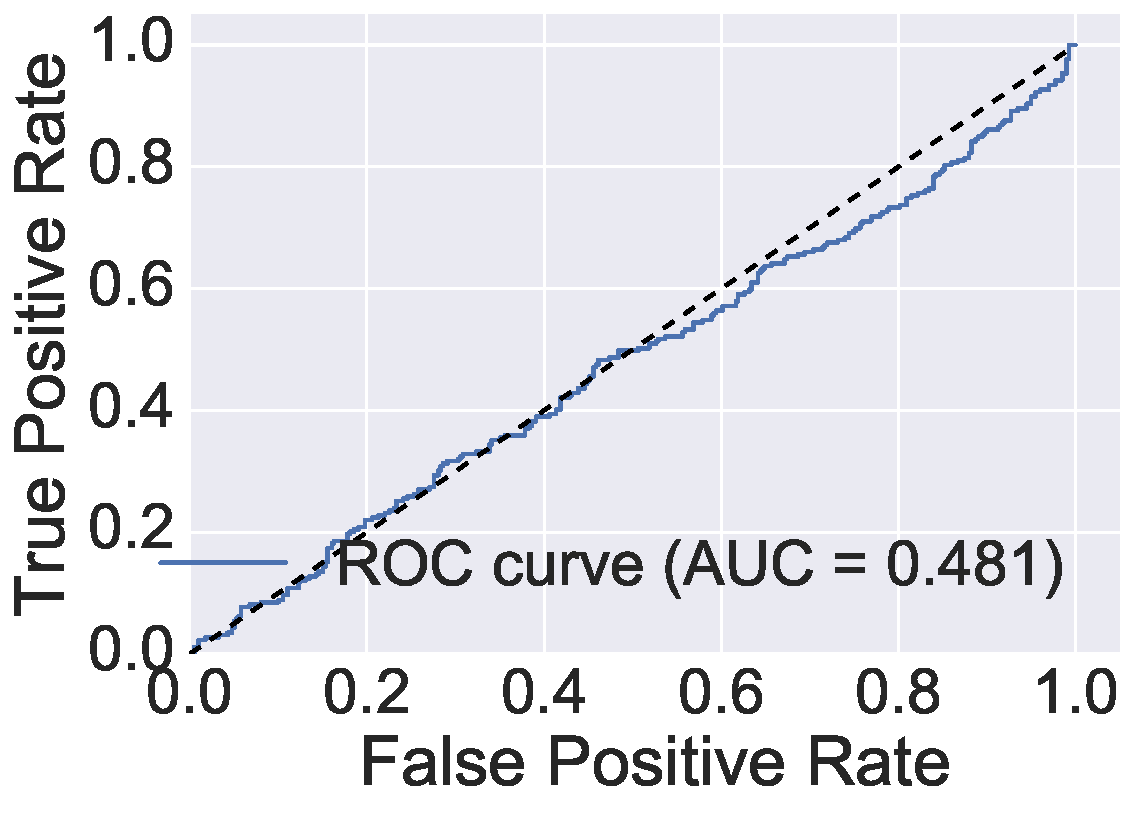
\includegraphics[width=.4\textwidth]{{/Users/ijoseph/Documents/Work/Graduate-Thesis/TeX/figures/ch4/cgp/log_reg_under_roc}.pdf}}%
      \qquad \\
      \subfloat[][Over-fit: $C = 1 \times 10^{15}$.]{
        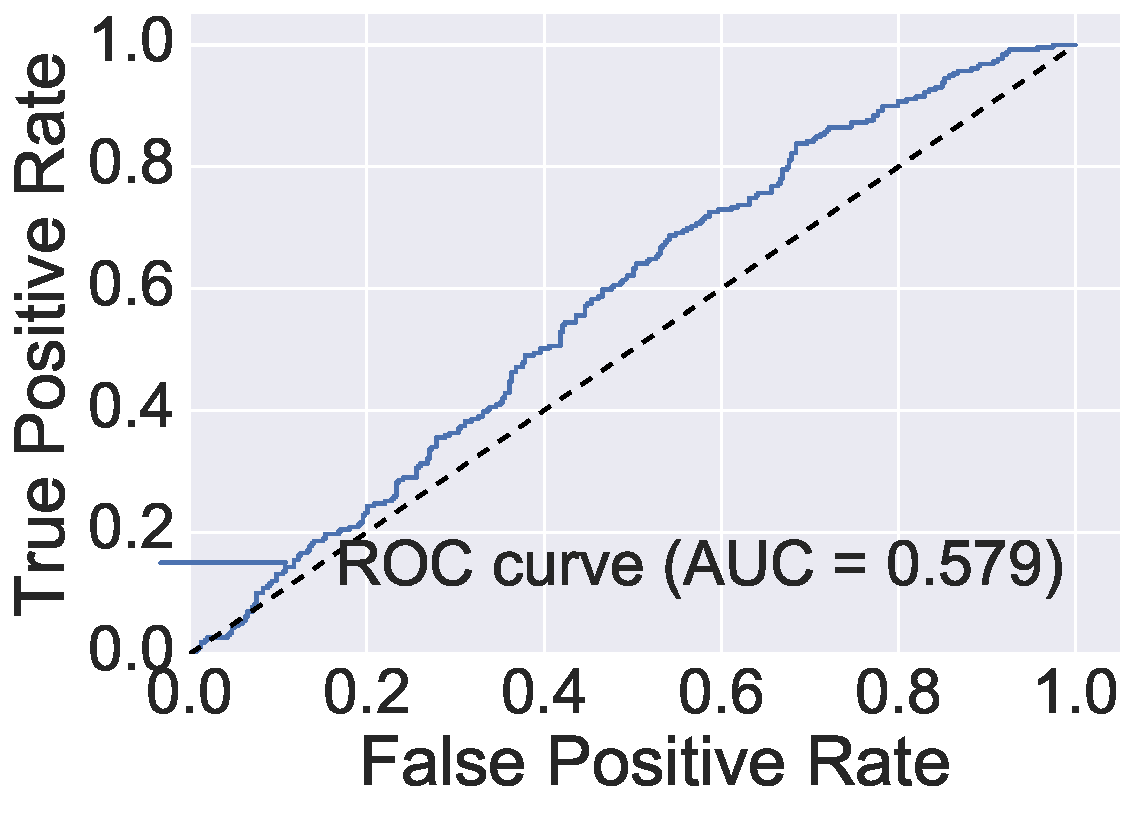
\includegraphics[width=.4\textwidth]{{/Users/ijoseph/Documents/Work/Graduate-Thesis/TeX/figures/ch4/cgp/log_reg_over_roc}.pdf}}%
      \caption{Logistic regression ROC curves for different levels of model
        complexity.} \label{fourcgptwo}
    \end{figure}

%% confusion

\begin{figure}
  \centering \subfloat[][Well-fit: $z_1 = 20, z_2 = 45$.]{\noindent
    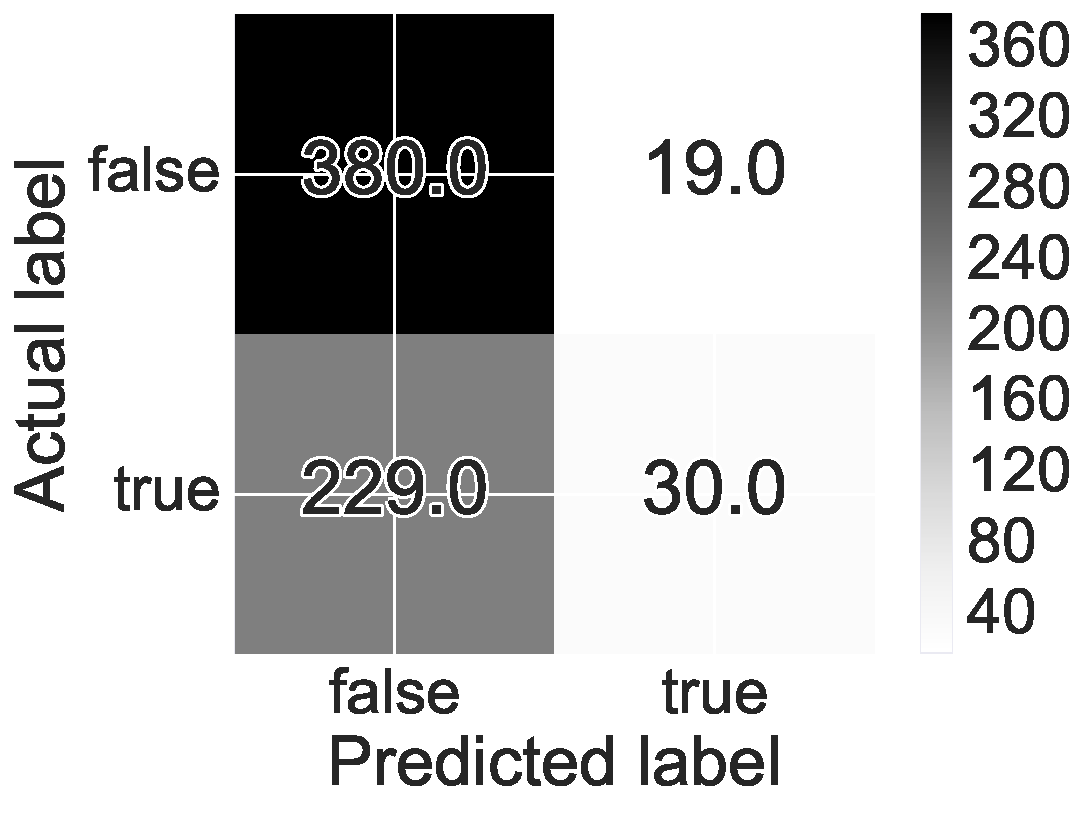
\includegraphics[width=.4\textwidth]{{/Users/ijoseph/Documents/Work/Graduate-Thesis/TeX/figures/ch4/cgp/mfaa_well_confus}.pdf}}%
  \qquad \\
  \subfloat[][Under-fit: $z_1 = 2, z_2 = 3$ .]{        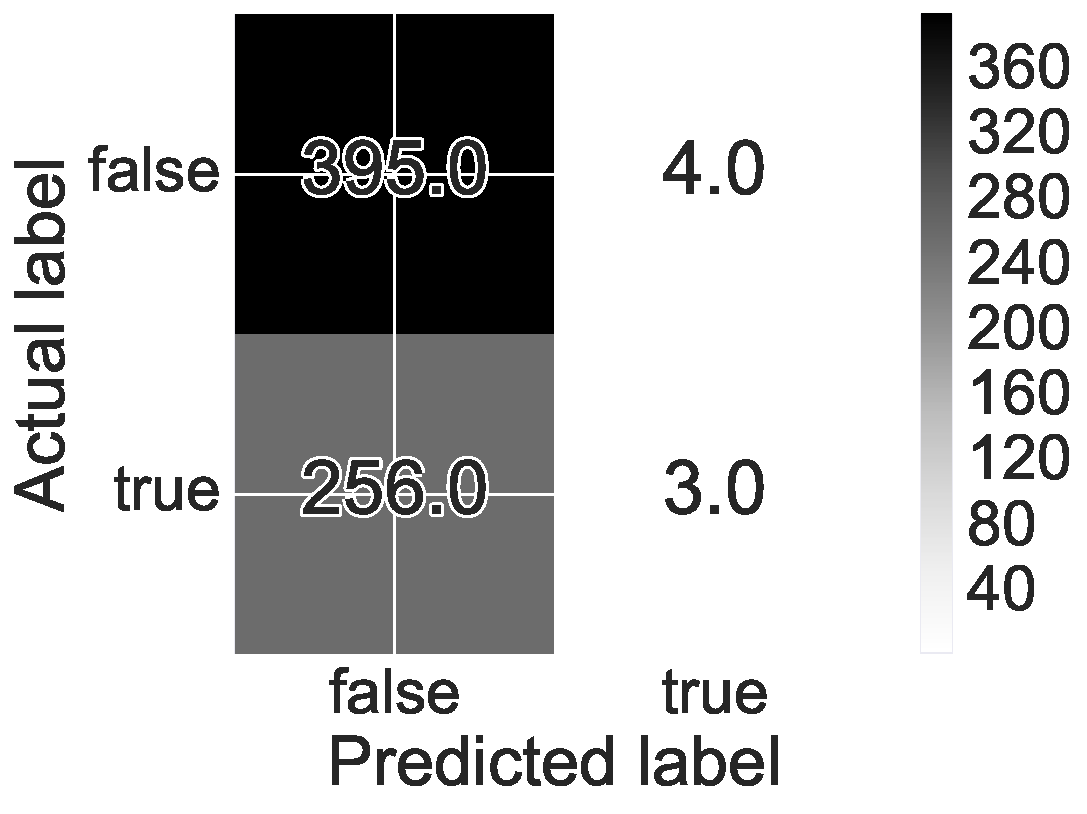
\includegraphics[width=.4\textwidth]{{/Users/ijoseph/Documents/Work/Graduate-Thesis/TeX/figures/ch4/cgp/mfaa_under_confus}.pdf}}%
  \qquad \\
  \subfloat[][Over-fit: $z_1 = 62, z_2 = 65$.]{        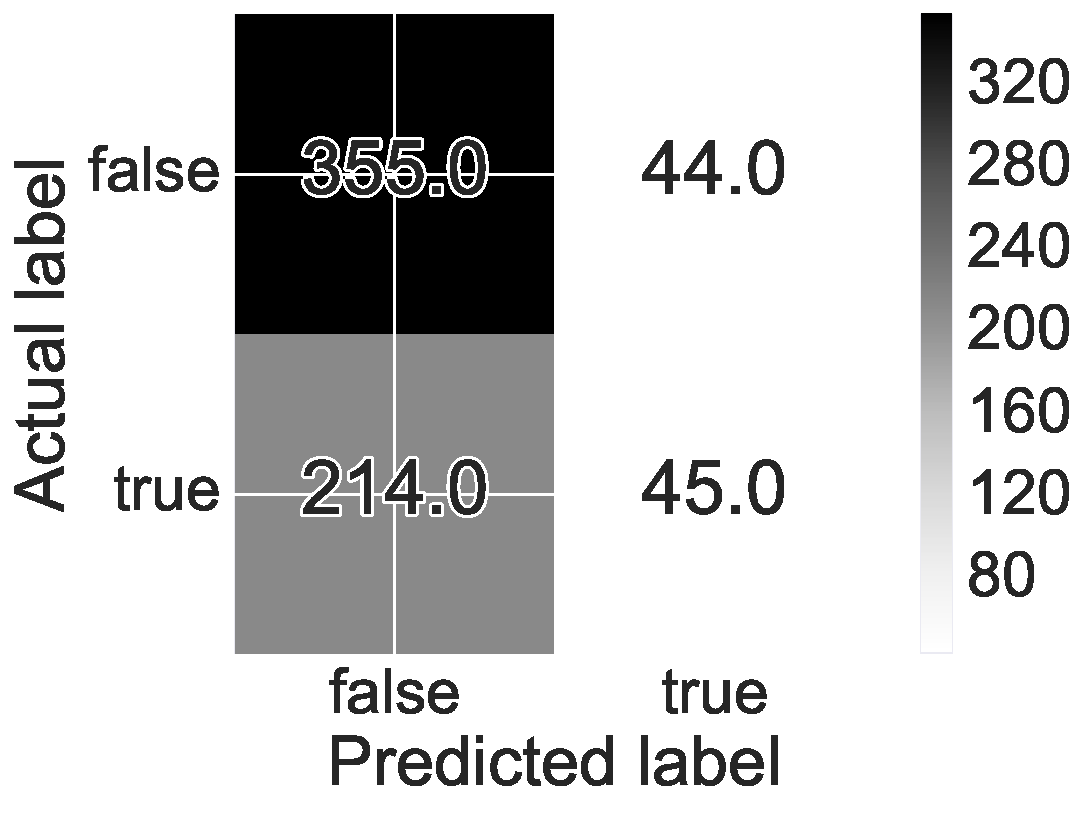
\includegraphics[width=.4\textwidth]{{/Users/ijoseph/Documents/Work/Graduate-Thesis/TeX/figures/ch4/cgp/mfaa_over_confus}.pdf}}%
  \caption{HFAM confusion matrices for different levels of model
    complexity.} \label{fourcgpthree}
\end{figure}
    

    \begin{figure} 
      \centering \subfloat[][Well-fit: $C = 1 \times 10^5$.]{\noindent
        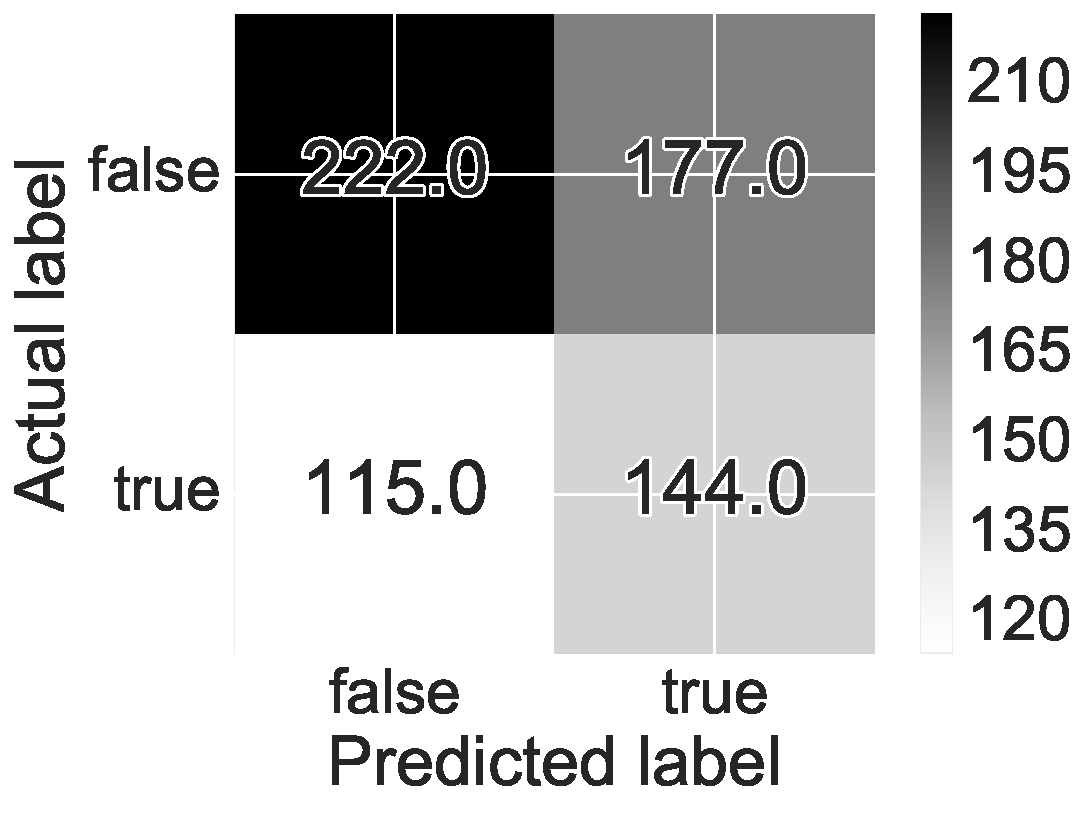
\includegraphics[width=.4\textwidth]{{/Users/ijoseph/Documents/Work/Graduate-Thesis/TeX/figures/ch4/cgp/log_reg_well_confus}.pdf}}%
      \qquad \\
      \subfloat[][Under-fit: $C = 1 \times 10^{-5}$
      .]{
        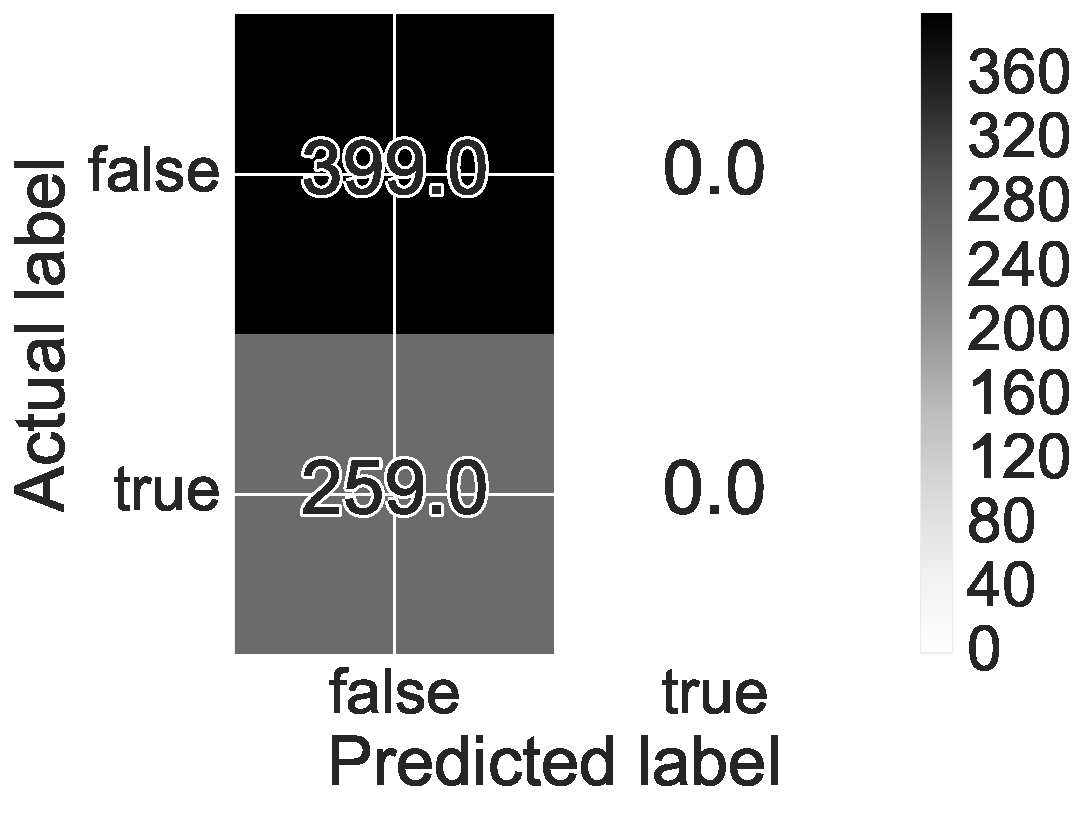
\includegraphics[width=.4\textwidth]{{/Users/ijoseph/Documents/Work/Graduate-Thesis/TeX/figures/ch4/cgp/log_reg_under_confus}.pdf}}%
      \qquad \\
      \subfloat[][Over-fit: $C = 1 \times 10^{15}$.]{
        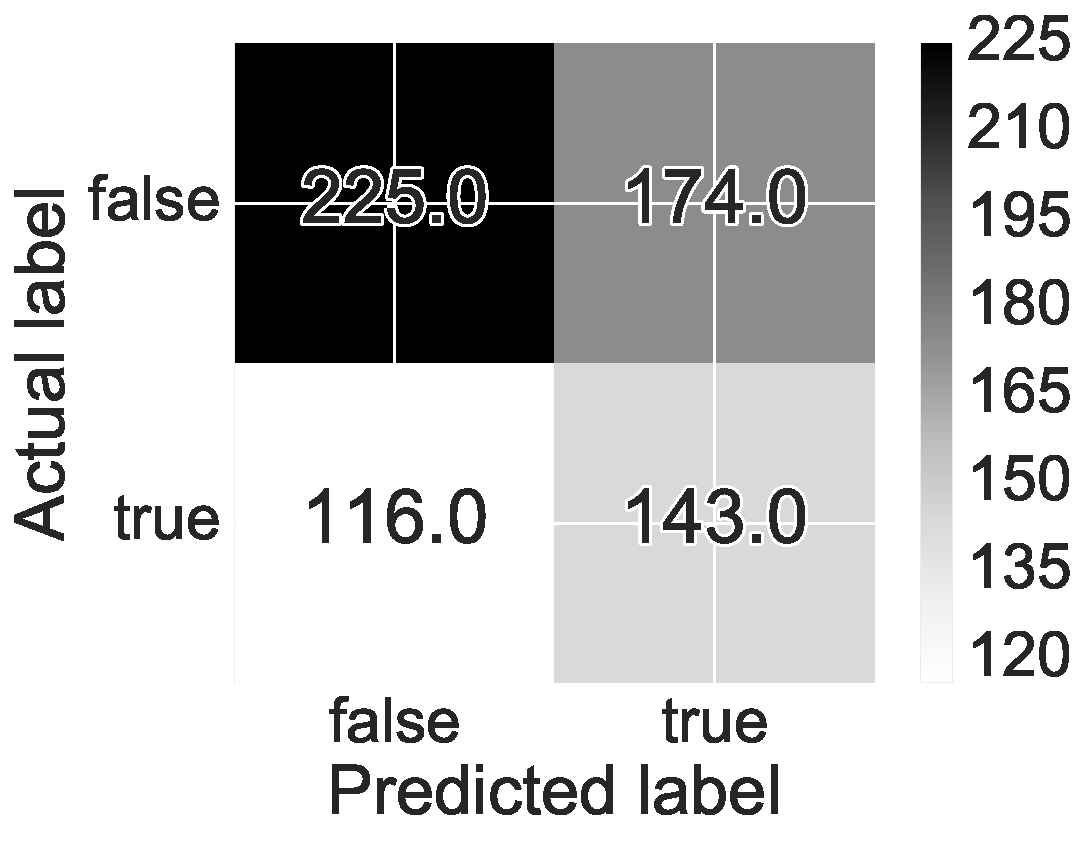
\includegraphics[width=.4\textwidth]{{/Users/ijoseph/Documents/Work/Graduate-Thesis/TeX/figures/ch4/cgp/log_reg_over_confus}.pdf}}%
      \caption{Logistic regression confusion matrices for different levels of model
        complexity.} \label{fourcgpfour}
    \end{figure}